\chapter{OpenStreetMap}% je videt
\label{2-OpenStreetMap}


\section{Vznik}
\label{vznik}
OpenStreetMap (OSM) je projekt, jež vznikl s cílem vytvoření a sběru 
volně dostupných geografických dat a následně jejich možné vizualizace
do topografických map. Projekt založil Steve Coast v červenci roku 
2004 v Anglii. Jako inspiraci mu byl projekt Wikipedia. 

Zprvu projekt využívalo jen pár nadšenců, ale postupem času získal 
projekt popularitu. S nárůstem počtu uživatelů narůstal i objem dat. 
Bylo tedy nutné zvyšovat kapacitu serverů. 

V dubnu roku 2006 byla založena nadace OpenStreetMap fundantion pro financováni 
samotného OSM (zaměstnanců, běhu serverů atd.). 
%\cite{wikiOSM}


\section{Struktura dat}
\label{struktura dat}

OSM data jsou ukládána ve formátu XML (verze 1.0). Jeho výhoda je jasná 
struktura, snadná orientace v kódu pro člověka. Nevýhodou je ovšem větší objem 
dat, který lze ale snížit kompresí. 

Každý prvek má vlastní XML soubor. 

příklad XML souboru pro linii:

{\scriptsize
\begin{lstlisting}
<osm version="0.6" generator="CGImap 0.4.0 (32632 thorn-01.openstreetmap.org)"copyright="OpenStreetMap and contributors" attribution="http://www.openstreetmap.org/copyright" license="http://opendatacommons.org/licenses/odbl/1-0/">
   <way id="87249754" visible="true" version="2" changeset="34489106" timestamp="2015-10-07T11:52:41Z" user="Petr Dlouhý" uid="17615">
       <nd ref="1014526199"/>
       <nd ref="1014525941"/>
       <nd ref="1014526337"/>
       <nd ref="1014526022"/>
       <nd ref="1014526277"/>
       <nd ref="1014525984"/>
       <tag k="highway" v="path"/>
       <tag k="source" v="bing:ortofoto"/>
   </way>
</osm>
\end{lstlisting}
}

Třídy prvků v OSM jsou rozděleny na uzel (node), cesta (way) a 
relace (relation).

Uzel je definován jedinečným identifikátorem ({\tt node id=}). Jeho 
souřadnice jsou ve WGS~­84. Je také ukládána verze (version) a kdy 
byl do databáze přidán a v jaké změně to bylo provedeno (changeset=). 
Dále k bodu je možná připojit různé atributy s klíčem a hodnotou (tag~
k=~~v=~~). 

Linie je spojení dvou a více uzlů a má taky svůj identifikátor (way~
id=). Hlavičku má shodnou s bodem. Ale obsahuje také seznam id uzlů, 
jež ji tvoří. Liniím lze jí taktéž přiřadit atributy.  

Linie lze ještě rozdělit na neuzavřené a uravřené. Uzaveným liniím lze připojit 
i atributy určené jen pro plochy. Například les (landuse=forest).
V případě, když přidává-li se atribut jež je v základu pro linieale chceme ho použít pro plochy přidává se atribut area=yes.

Speciálním příkladem jsou relace (relation=*), do které lze zahrnout 
jeden a více prvků. Lze do nich spojit prvky stejné nebo odlišné třídy 
nebo i jiné relace. Pro příklad dálnice je tvořena mnoha liniemi a ty 
jsou zahrnuty do společné relace Dálnice D1. Nebo turistická trasa 
(od~KČT) je relace sdružující linie (cesty, pěšiny) tak i uzly 
(rozcestníky, vyhlídky, apod. ).

U atributů popsaných na osmwiki je vždy uvedeno, k jaké třídě je 
vhodné a nevhodné je použít (dle komunity uživatelů OSM). Pokud se stane, že je použit 
na~jinou než povolenou třídu, nemusí to hlásit chybu, ale může být následně 
problém v některých vykreslovačích. 

\section{Licence}
\label{licence}

Původní data OSM byla na distribuována pod licencí 
Creative~Commons~Allribution­Share~Alike 2.0 (CC~BY~­SA~2.0). 
(Lincence CC~BY~SA~2.0 zní:  „ ... “  )

Tato licence umožňovala užití (distribuci ale i editaci) díla pod podmínkou, 
že bude uveden zdroj OpenStreetMap.org ve viditelné části 
vytvořených mapových dlaždic [?2] 

  \begin{figure}[hbt]
    \centering
      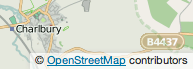
\includegraphics{./pictures/attribution_example.png}
      \caption{attribution example}
      \label{fig:attribution_example}
  \end{figure} 

Roku 2012 byla licence publikovaných dat změněna na Open Data Commons 
Open Database Licence (OdbL). Tato změna licence přinesla problém 
s~daty, které byly poskytnuty projektu v předchozí licencí 
(CC­~BY~SA~2.0). Bylo nutné se dotázat každého z dřívějších 
přispěvatelů dat, ať už právnických osob tak i fyzických osob, jestli 
s touto změnou souhlasí a je možné s jejich daty i s novou licencí 
nakládat. U přispěvatelů, kteří nedovolili užívání jejich díla 
pod novou licencí, nebo u těch, co se nevyjádřili, bylo nutné 
z~databáze vymazat. Tato situace nastala pouze ve zlomku případů. 
Nejvíce tato změna licencí ohrozila data v zemích jako je Polsko a Nový Zéland.
 [?5] 

\section{Opendata}
\label{opendata}
Základní myšlenka otevřených dat vznikla v USA z iniciativy vlády Barracka Obamy. 
Tedy, pokud vzniknou geografická data z veřejných peněz, měla by tedy být přístupná 
veřejně. Mělo to kladný efekt na tamní ekonomiku.
Díky tomuto byly zprvu k dispozici satelitní snímky povrchu 
Země a digitální model terénu s rozlišením 30x30 m od NASA (pro 
pozdější vykreslení vrstevnic). 

Tento trend se začal rozšiřovat zprvu do zemí západních Evropy,
jmenovitě Anglie, Francie, ale i jiné země mimo Evropu..  

V ČR se tomuto věnuje fond otevrenadata.cz, který založil Otakar 
Motejl. Teto fond spolupracuje s nadací Sociery Fund Praha. V rámci 
těchto uskupení je vyvíjen tlak na zveřejňování smluv a dat 
státních institucí, jelikož jejich získání a údržba bylo placeno 
z~veřejných zdrojů.

\section{Zdroje dat}
\label{opendata}

Jak bylo zmíněno, byla snaha aby mapová data tvořili jedinci, vlastním 
sběrem dat. Sběr dat ve smyslu měřením vlastní GNSS (GPS, Glonass) 
přijímačem a znalost místních poměrů (uzavřené silnice, stezky atd.). 
Toto mapové dílo z těchto dat mohli volně užívat k vlastním užití. 
Komunita přispěvatelů se zprvu pomalu, ale později rychle rozrostla a 
dnes čítá 3,7 milionů registrovaných uživatelů s alespoň jednou 
vytvořenou změnou v OSM a 2,7 milionů účtů aktivních přispěvatelů.

Tyto mapové podklady byly velice vhodné i pro další projekt, dnes již 
velice rozšířený a známý jako Geocashing (GC). Projekt GC začal mapové 
podklady od OSM užívat a zároveň jeho uživatelé začali sami tvořit a 
přispívat do OSM. 

Přispěvatelé dat do OSM musí respektovat, že OSM je pod licencí OdbL. 
Tudíž i jejich zdroj dat musí splňovat tuto licenci. Proto by měli 
všechny svoje změny, které v OSM vytvoří, řádně ozdrojovat atributem 
s~klíčem 
source=*
V případě vlastním sběrem dat se vyplňuje hodnotou 
source=survey
případně uvést zdroj, odkud čerpali. Pokud tuto povinnost poruší a 
použijí zdroj, jež není kompatibilní z politikou OSM, tak samotné OSM 
jejich změnu, aby předešel sporům, sám vymaže. Bohužel musí vymazat 
celou sadu změn, byť by v něm byl jeden prvek, jež toto poruší. 

Druhým významným zdrojem dat jsou soukromé subjekty (společnosti). 
V~tomto případě jde většinou o podkladové zdroje dat. Pro obkreslování 
silničních síti z~leteckých nebo satelitních rastrů. V~jejich případě 
řešeno písemným svolením, nebo smlouvou. Jako významným zdrojem byla 
společnost Bing, jež nabídla k~dispozici letecké snímky většiny 
obydlené pevniny. 

Třetím zdrojem a zároveň postupně dominujícím co do obsahu dat, jsou 
databáze ze státního sektoru. Tyto databáze jsou nejvhodnějším zdrojem 
dat. Data v nich jsou důkladně spravována už proto, že je využívá stát. 

\section{Vykreslovače}
\label{vykreslovače}
Na hlavní stránce OSM je pět „základních“ přednastavených vrstev vykreslených 
z~dat z OSM. Využívá aplikaci OpenLayers založenou na konceptu AJAX.

\begin{itemize}

  \item Standardní vrstva - vykresluje všechny prvky přiměřeně.
  \item Cyklomapa - vykresluje cyklostezky, výškopis. 
  \item Dopravní mapa - vykresluje silniční a železniční sítě.
  \item MapQuest Open vznikla jako podkladová mapa právě pro potřeby 
Geocaching.
  \item Humanitární mapa, která vykresluje služby (restaurace, banky, muzea, 
  školy, kostely...)  a potlačuje ostatní prvky 

\end{itemize}

Existují další stránky jež se zabývají vlastní kompozicí a vykreslením
různých dat. Například mapu turistických a cyklistických tras vykresluje
 mtbmap.cz a to pro celou Evropu. 
 
Zajímavými projekty jsou, které k 2D mapě přidává „třetí“ rozměr a 
vytváří tzv. 2.5D mapu. Většinou jde o 3D zobrazení budov, mostů (dle 
atributů) popřípadě i stromů. 

